
\section{Virtual Audit System:}

\indent We present a Virtual Audit System for residential buildings to identify the causes for HVAC energy waste and provide proper feedback to customers. Two important factors for energy waste are poor building construction and bad thermostat settings. If a house has poor thermostat settings, then the utility providers can provide feedback to adjust setpoints. On the other hand, for the homes which are have poor construction, we can provide a detailed diagnostic for a home to isolate the constructional reasons behind abnormal usage.

\subsection{Building Parameter Identification:} 

 \indent Building construction materials can be the potential determining factors for energy usage. Identifying building characteristics like insulation or resistance of walls and thermal mass or capacitance are the factors which has effect on the rate of heater/AC cycles being used. We investigated the techniques mentioned in~\cite{building} to find the greybox models for a building. A building heat consumption can be represented by an equivalent electrical circuit for which the equivalent state space equations are derived. With the fewer number of input parameters shown in the work its difficult to get a fully detailed model. We compare the state space model based parameter estimation with Kalman Filter against a proposed discriminative regression learning based approach.\\
 \indent The equation relating thermal energy to thermal mass is given as $Q = C \Delta T$, where where $Q$ is the thermal energy transferred, $C$ is the thermal mass of the building, and $\Delta T$ is the change in temperature. Finding the thermal mass will help compare buildings. Apart from the thermal mass the resistance or conductance of a building is a measure for insulation. We begin our investigation with a simple model for a house where we consider only two components of the circuit conductance(R) and thermal mass(C). The exact solar radiation can't be quantified without exact sensor data so we begin our study to find alternative approaches to modeling the building heat dynamics. The heat dynamics of the is given by the state space equations as follows - 
 
 \begin{eqnarray}
 \frac{dT_i}{dt} = \frac{1}{C  R} (T_a-T_i) + \frac{1}{C}\Phi_h + \frac{A_w}{C} \Phi_s + \sigma_i \frac{d\omega_i}{dt}\\
 Y_{i,t} = T_{i,t} + \epsilon_t
\end{eqnarray}  

 \begin{table}[t]
  \scriptsize
 \begin{tabular}{||c| c | c | c | c | c ||} 
 \hline 
 HomeID &  GAM & GLM & EKF & C & R  \\ [0.5ex] 
  \hline \hline
94 & 0.008  & 0.026  & \textbf{0.006 } &  14.556 &
 0.386 \\ \hline 
410 &  0.009 & 0.009  & \textbf{0.008} &  33.858 &
 0.595 \\ \hline
484 & 0.007 & \textbf{0.007} & 0.007 &  108.078 &
 0.472\\ \hline
871 & 0.010  & \textbf{0.010 } &  0.011 & 20.633 &
0.874\\ \hline
1314 & 0.006   & \textbf{0.006 } & 0.007 & 1092.865 &
0.019\\ \hline
1507 & 0.008  & \textbf{0.008 } & 0.009 & 257.370
& 0.1507 \\ \hline
1714 &  0.011  & \textbf{ 0.011 } & 0.013 &  72.967 & 
 0.191\\ \hline 
2470 & 0.009  & 0.009  &  \textbf{0.009} & 101.546&
1.232\\ \hline 
2814 & 0.008 & \textbf{0.008} & 0.009&  60.881&
 0.183\\ \hline
3367 & 0.007 & \textbf{0.007} & 0.007 & 944.656
& 0.130\\ \hline
5371 & 0.023 & 0.023 & \textbf{0.0208} &  80.065 & 
 0.284\\ \hline
6673 & 0.0074 & \textbf{0.0074} &  0.0074 &90.806
&0.348\\ \hline
7989 & 0.003 & \textbf{0.006} & 0.010 &16.215
&0.289\\ \hline
8600 & 0.009 & \textbf{0.009} & 0.010 &934.0354
&0.038\\ \hline
 \hline
\end{tabular}
 \label{Table:Par1}
\caption{Comparative Results of Parameter Estimation and Building Modeling on Pecan Street Data(NMSE)}
\end{table}
  
  
 \indent The equations (2) and (3) are the state-vector equations and the measurement equations respectively. The thermal resistance is given by R and the thermal mass by C. More detailed thermal mass and resistance for building materials can be obtained where the individual thermal mass can be taken under consideration like that for building envelope, the walls and furniture etc. We found that the simplest model can be exactly achieved with slightly better residual loss using a regression model - (Generalized Linear Model(GLM)). One of the advantages of GLM is the training process is simpler and it is easier to model and represent abstract information for example cloud cover and time of day features and help construct a discriminative model. \\
 \indent The state space equation can be discretized as \begin{eqnarray}
 \frac{dT_i}{dt} = \frac{1}{CR} (T_a-T_i) + \frac{1}{C}\Phi_h + \frac{A_w}{C} \Phi_s + \sigma_i \frac{d\omega_i}{dt} \\
  T_i(t+1)  = (1 - \frac{1}{CR}) T_i(t)+\nonumber \\  (\frac{1}{C}\Phi_h(t) + \frac{A_w}{C} \Phi_s(t) + \frac{1}{CR}T_a(t))\\
   T_i(t+1)  = c_1 T_i(t)+   c_2\Phi_h(t) + c_3\Phi_s(t) + c_4T_a(t) + \epsilon \nonumber \\
   1 - C_1 = C_4 \label{eqn:Reg}
\end{eqnarray}  
  
  
 \indent The discretization of the state space equation gives us an approximate equation which is given in Eqn~\ref{eqn:Reg}.  This can be seen as a constrained regression equation and instead of using the a complex Extended Kalman Filter based approach we can solve it using regression techniques.  We compared the errors in residuals among Extended Kalman Filter(EKF), constrained Generalized Linear Model(GLM) and Generalized Additive Model(GAM). We found that the GAM gives comparatively less error in estimation than either of them as shown in Table~\ref{Table:Par1}. We compared regression models in Table~\ref{Table:Par1} and found that GLM gives us better results for most of the cases. While GAM outperforms the rest some of the times, it is easier to obtain the co-efficients from GLM. We also list the parameters Thermal Mass(C) and Insulation(R) for each of the homes. While CTSM outperforms GLM some of the times, its mostly for smaller datasets and it even fails to converge sometimes if the data is too large.  A sample output showing the residuals of CTSM and GLM has been shown in Figure~\ref{img:resid}. 
 
\indent The main dataset for comparison is Pecan Street's Dataset. We found that the regression models perform better for them than the CTSM model which results in high residual errors for this dataset. The other problem is CTSM seems to work better for smaller samples while more parameters can be added in case of GAM models where in case of absence of certain parameters like Solar radiation complex features like Time of Day, Cloud cover etc. can be added.  Also, the initialization for the parameters require specification of the range of values for the parameters need to be specified. CTSM suffers from convergence error on large datasets, like that from Pecan Street Dataport.

  
\indent \textbf{Thermal Mass Metric:} Thermal Energy of a house is theoretically quantified as the product of the Thermal Mass and the change in temperature which is the energy loss for a particular change in temperature. This is a better metric for comparison and can be better evaluated from the dataset. So the time to heat or cool a house upto a Thermostat setpoint and also the heat dynamics during non-heating hours can be used as two different metrics for comparative purposes. One of the drawbacks of these methods is the reliance on indoor temperature for model development which may not be available all the time. Rather it's easier to obtain the Thermostat Metrics which are the different durations in which thermostat settings are changed and the setpoints of those settings. In the next section, we investigate the different approaches to find the Thermostat Metrics. While the capacitance and resistance provide a vague idea regarding building parameters it does not provide the idea about any comparative basis regarding how long it takes to heat or cool a house and how long it can retain or lose heat. In~\cite{ThermalMASS}, provides a similar take on Thermal Mass Metric however the metric requires data regarding building construction material. It mentions about the charge and discharge of thermal mass relative to season, which is heatiy cooling down the mass on a summer night and warming it up on a winter day. Hence the metric should address both the abilities. Apart from temperature more parameters can be taken into consideration like humidity, cloud cover and wind speed as that may have influence on user comfort. 
 
\begin{figure*}[!t]
 \centering
    \subfloat[Comparative plot of the residuals obtained using CTSM and GLM]{
        \label{img:resid}
        %\subcaption{House 2470: $T_a$,$T_i$ \& $\dc$}
        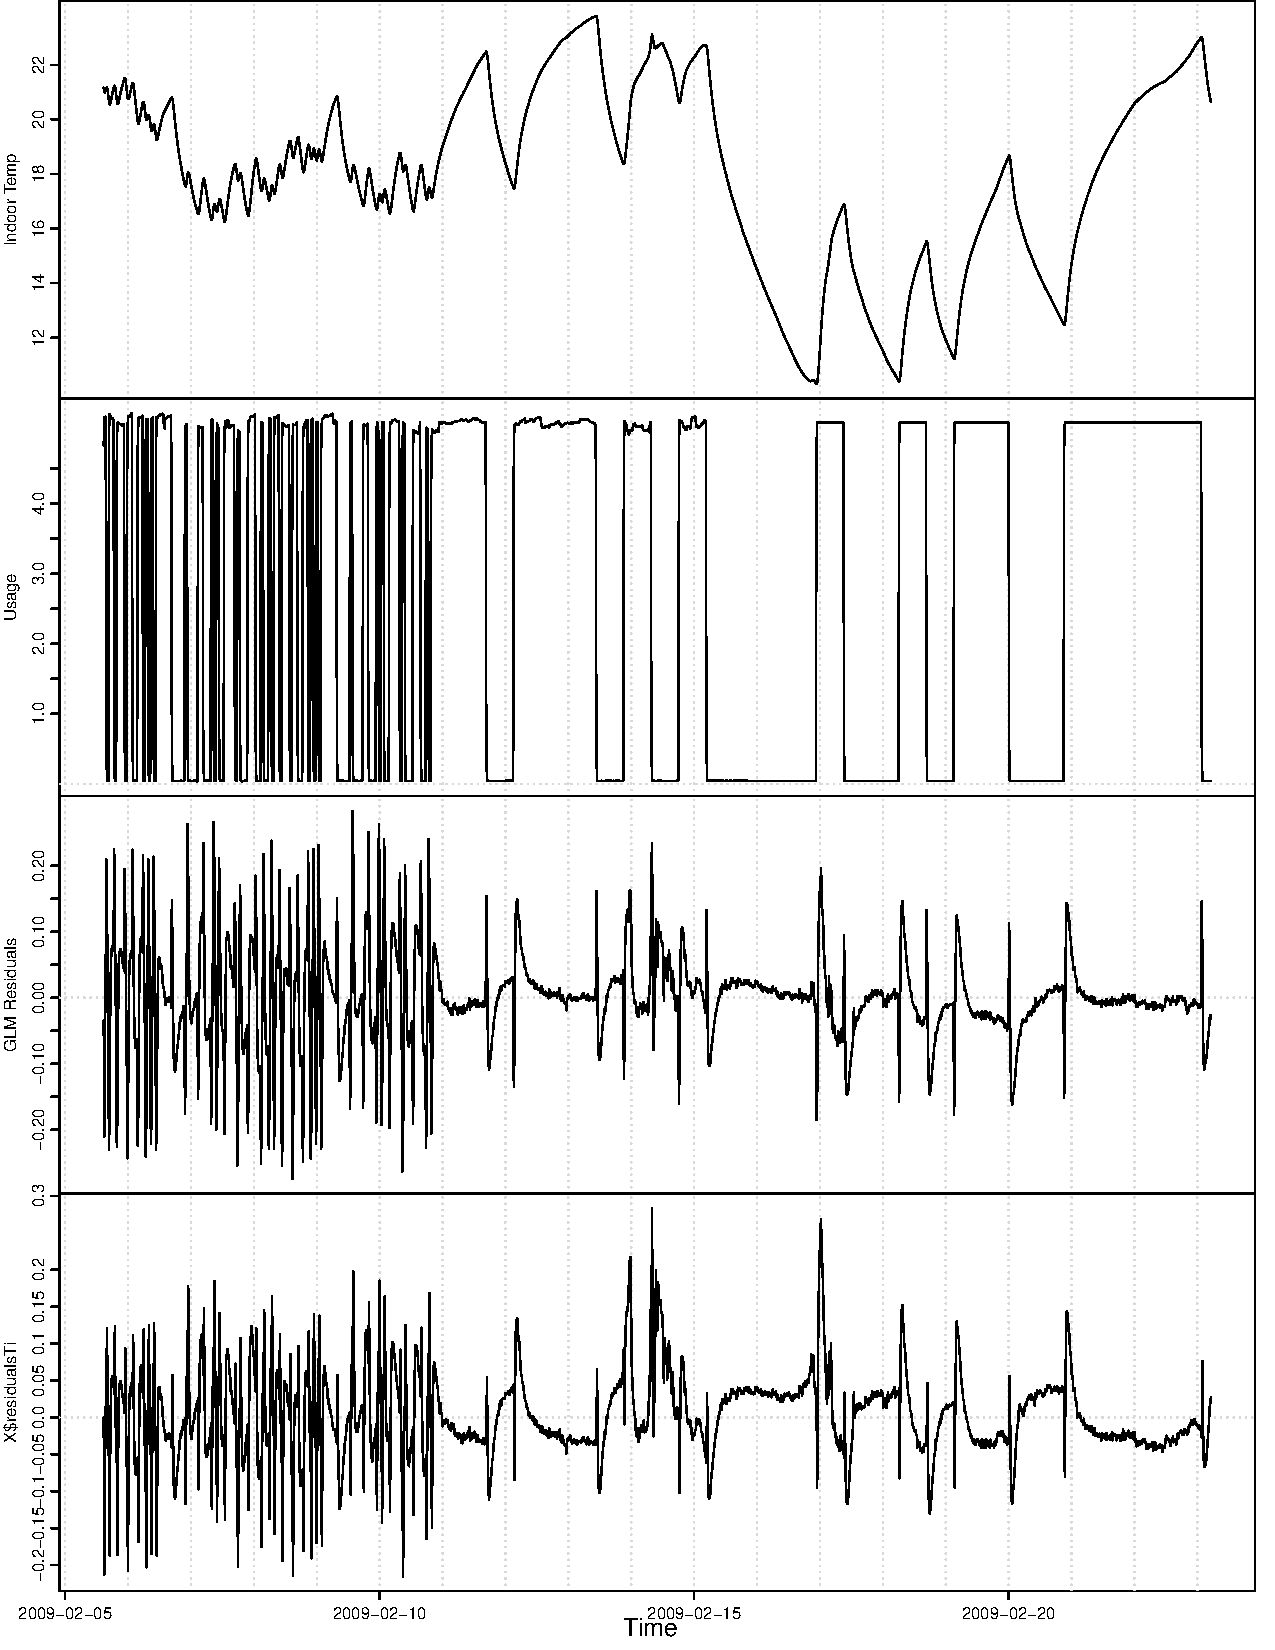
\includegraphics[height=3.6cm,width=3.2cm]{RplotResiduals}
    }\hspace{.7cm}
    \centering
     \subfloat[House 2470. $T_a$, $T_i$, dc]{
        \label{fig:subfig1}
        %\subcaption{House 2470: $T_a$,$T_i$ \& $\dc$}
        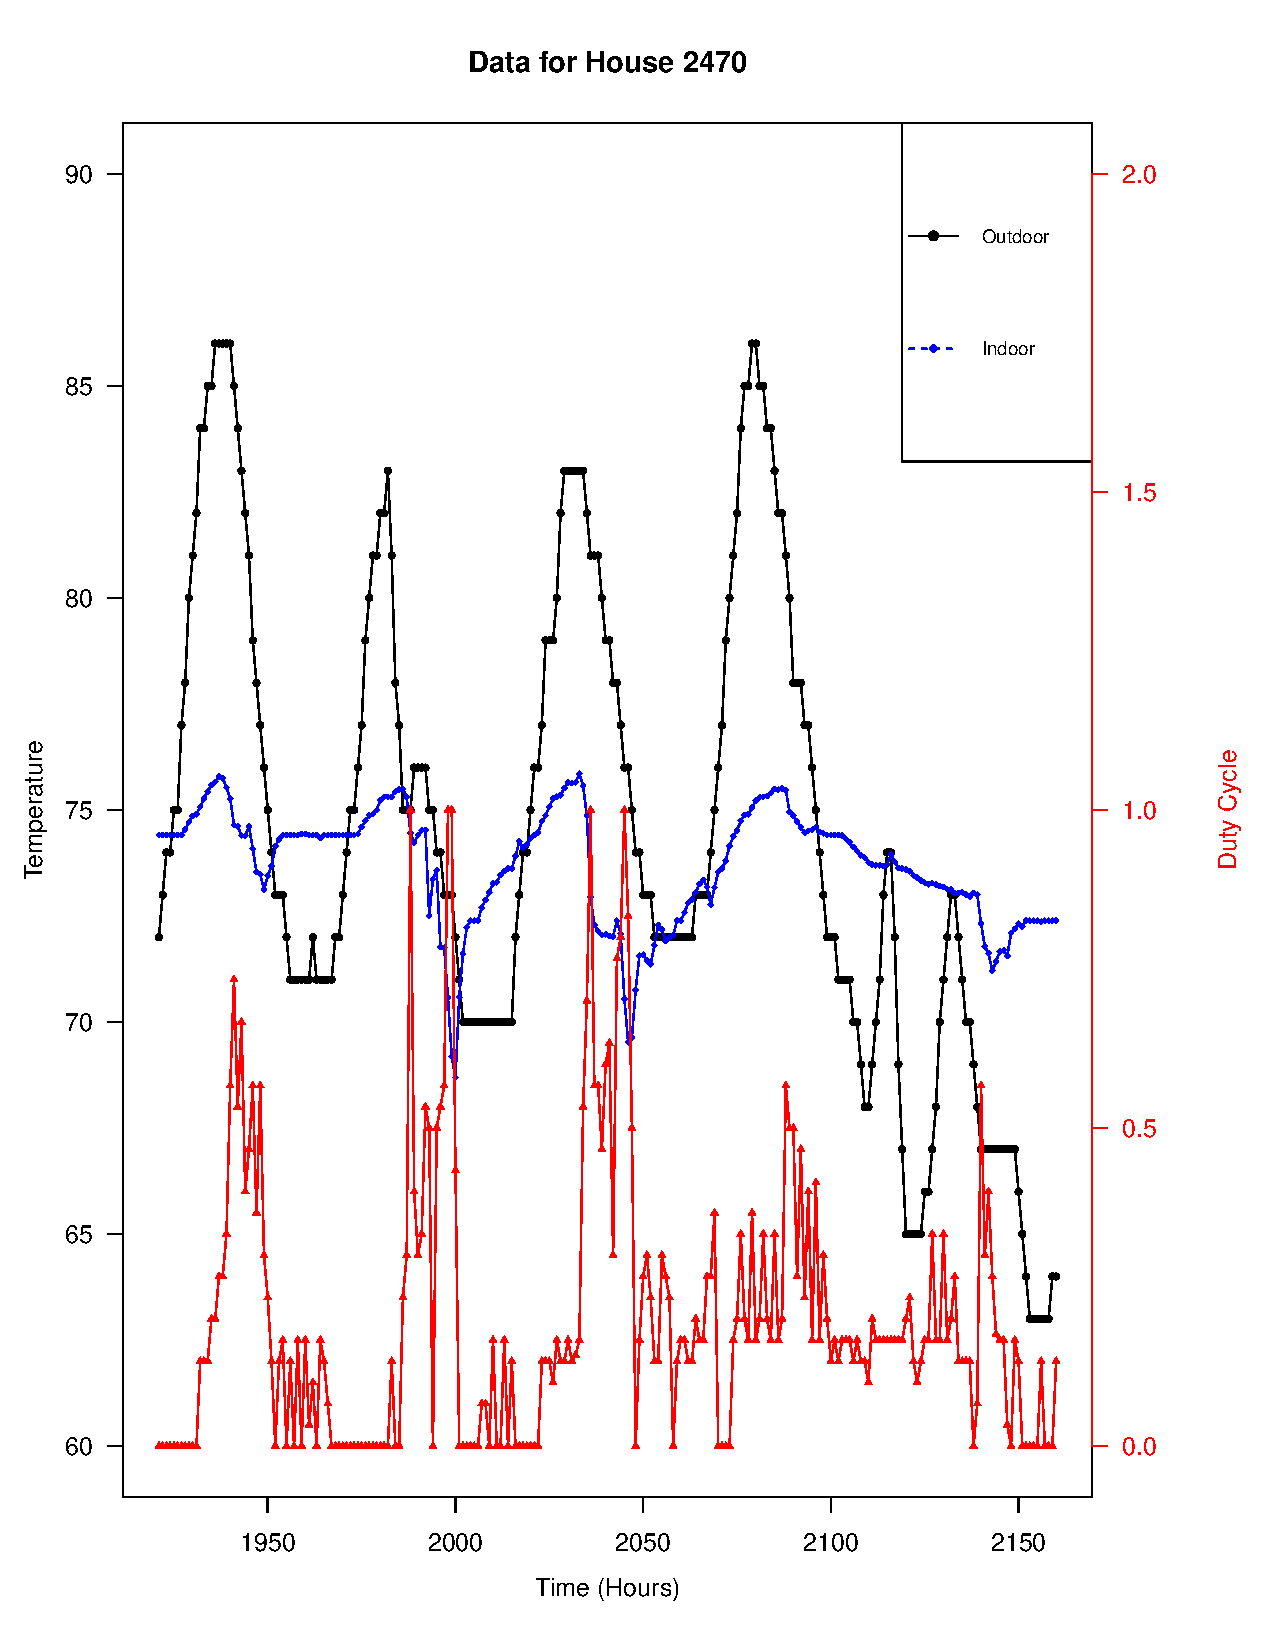
\includegraphics[height=4cm,width=4cm]{house2470}
    }
     \subfloat[ACF for a single day House 2470.]{
        \label{fig:subfig2}
       % \subcaption{ACF for a single day House 2470}
        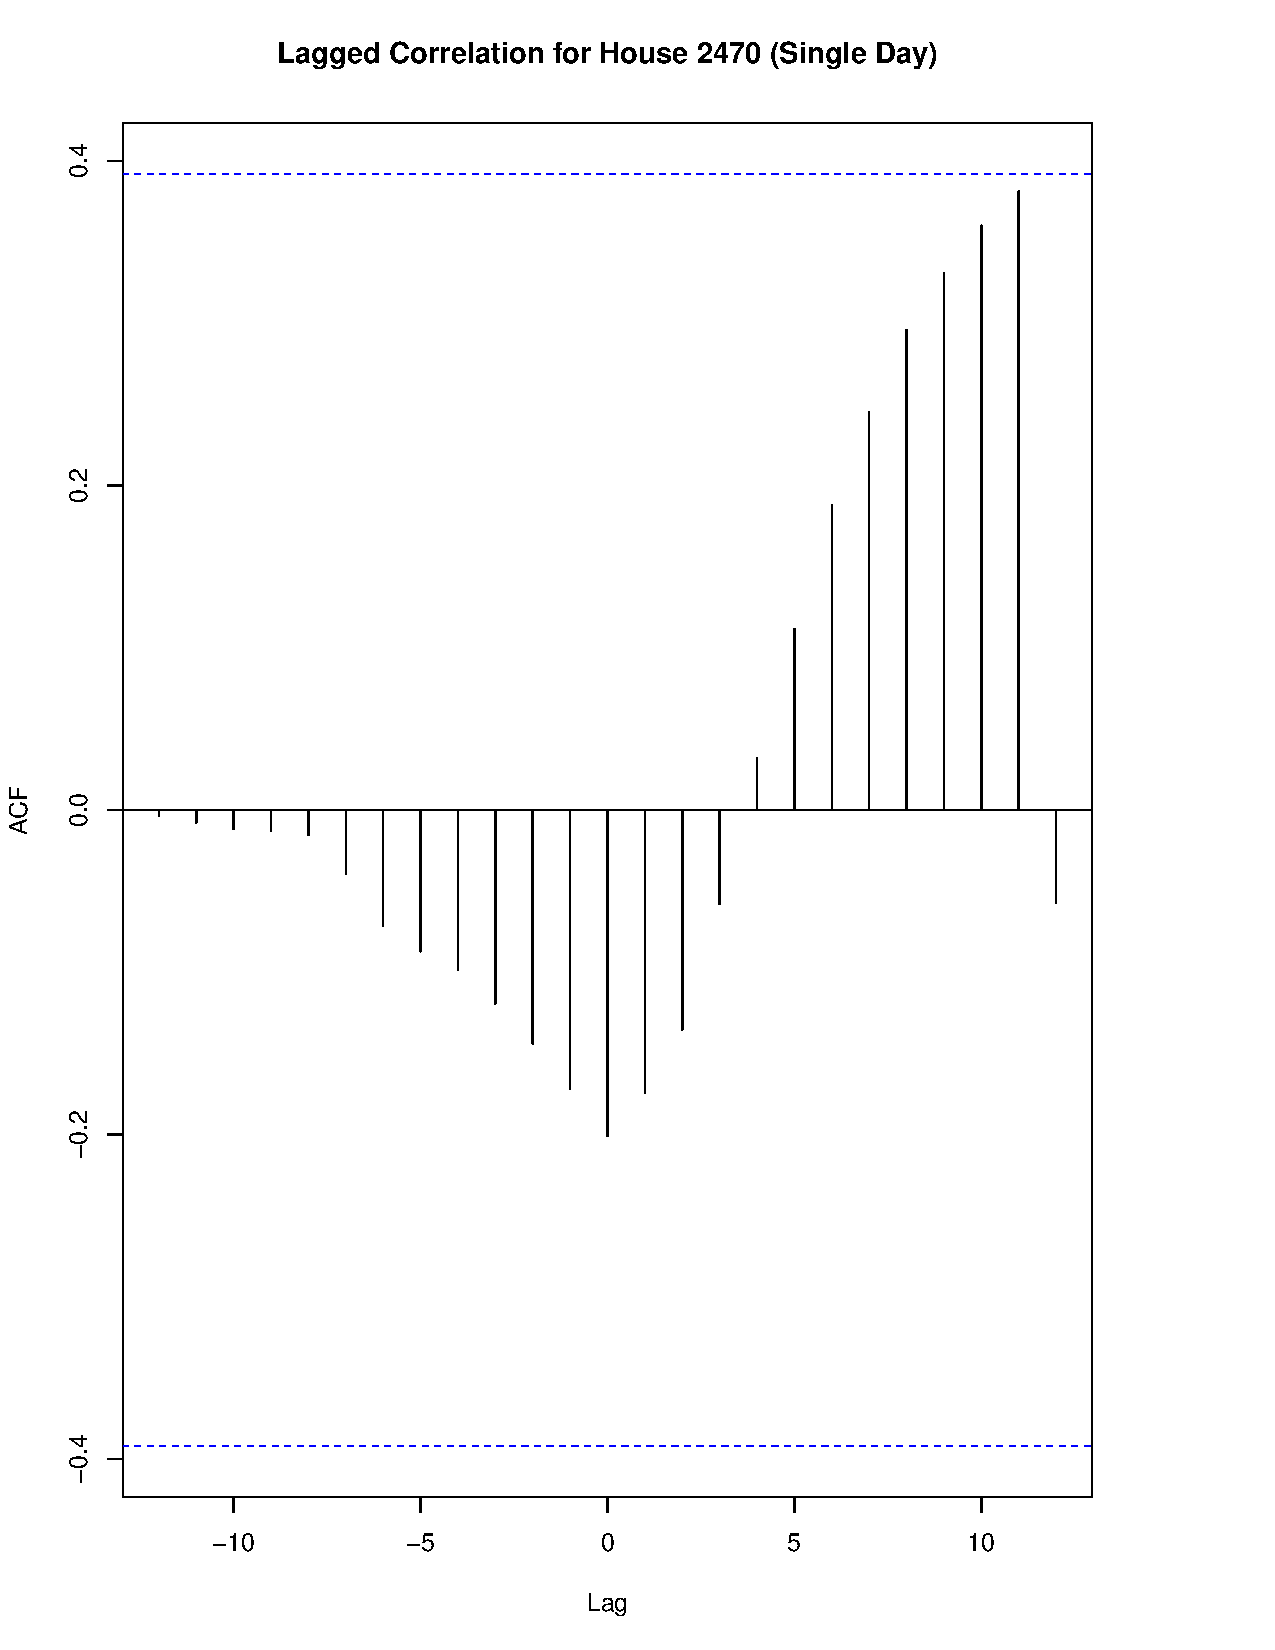
\includegraphics[height=4cm,width=4cm]{CCF2470}
    }
     \subfloat[House 410. $T_a$,$T_i$, AC, Heater]{
        \label{fig:subfig1}
       % \subcaption{House 1507. $T_a$,$T_i$, $\dc$}
        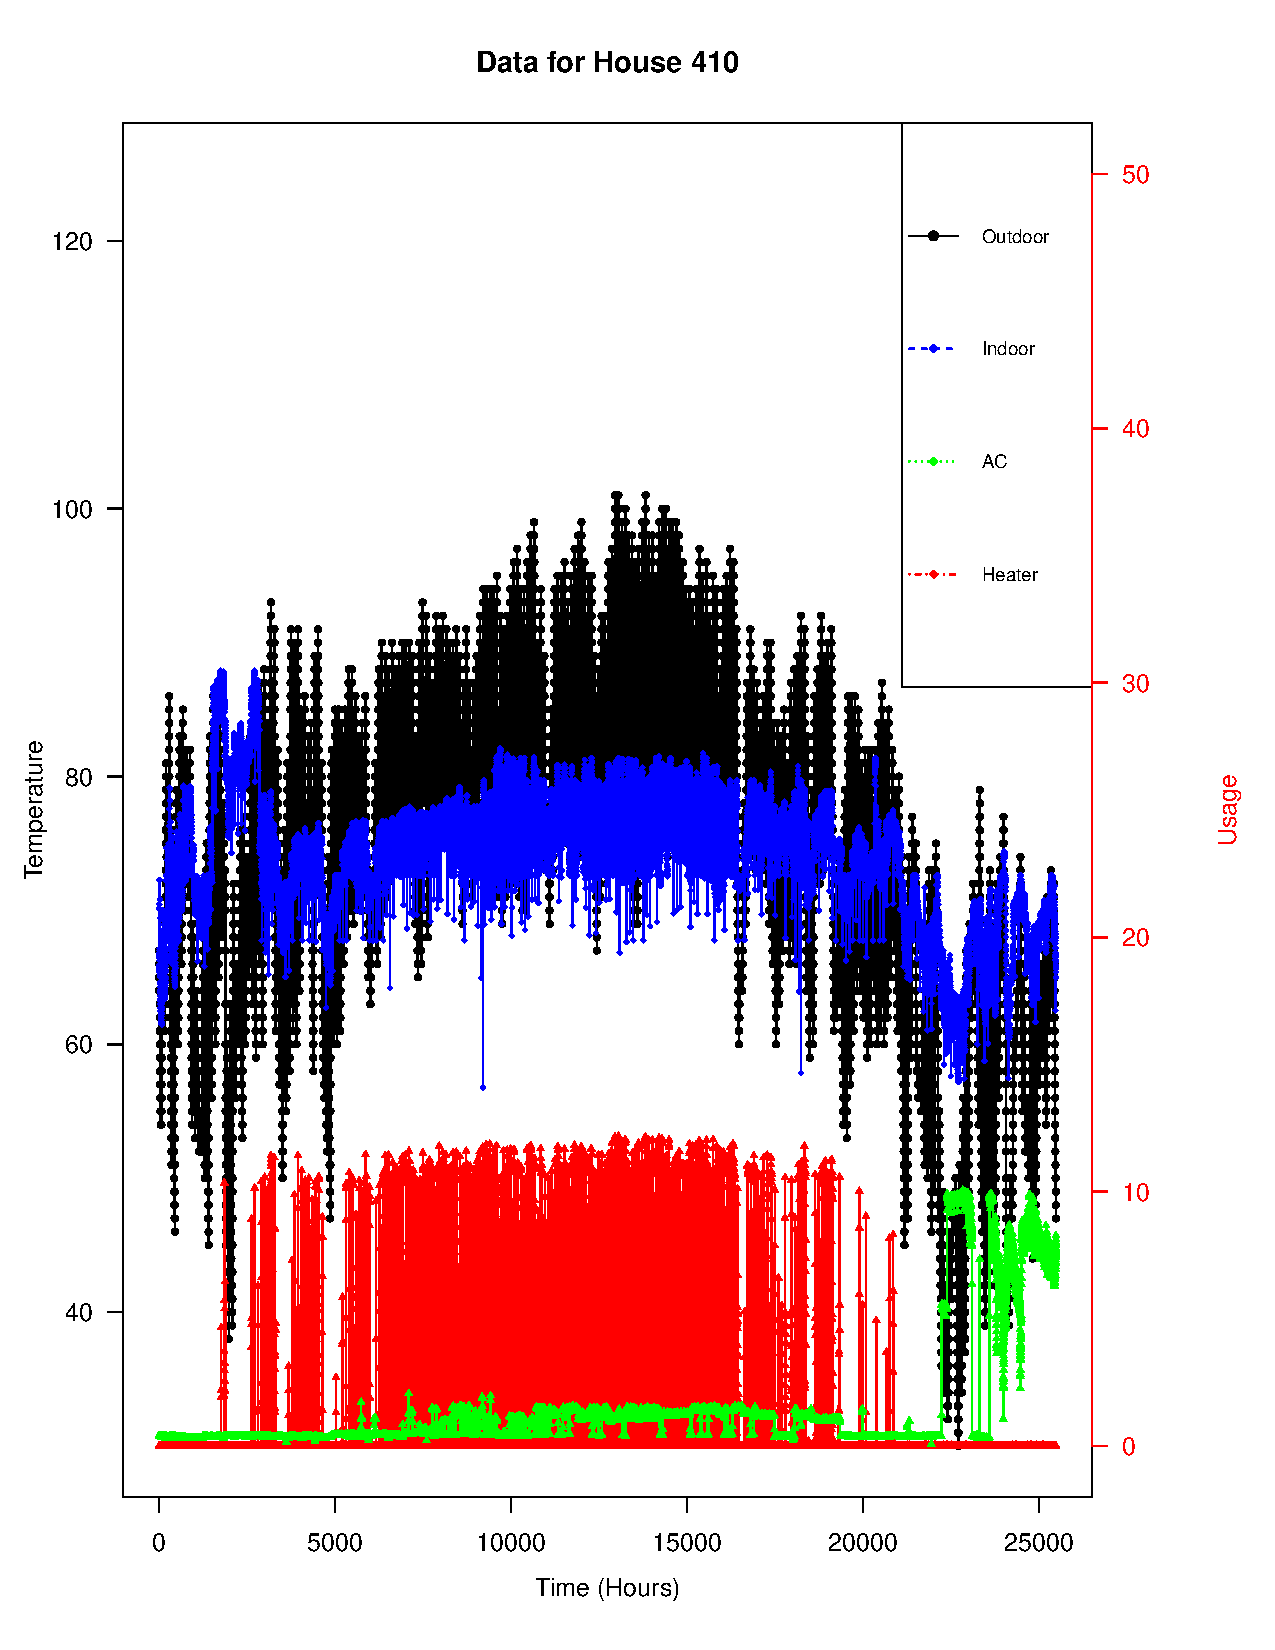
\includegraphics[height=4cm,width=4cm]{House410}
    }
    \caption{Sample Dataset of two homes}
    \label{fig:subfig}
\end{figure*}
